\documentclass[a4paper]{article}

% --- Packages ---

\usepackage{a4wide}
\usepackage[utf8]{inputenc}
\usepackage{amsmath}
\usepackage{mathtools}
\usepackage{amssymb}
\usepackage[english]{babel}
\usepackage{mdframed}
\usepackage{systeme,}
\usepackage{lipsum}
\usepackage{relsize}
\usepackage{caption}
\usepackage{tikz}
\usepackage{tikz-3dplot}
\usetikzlibrary{shapes.geometric}
\usepackage{pgfplots}
\usepackage{pgfplotstable}
\pgfplotsset{compat=newest}%1.7}
\usepackage{harpoon}%
\usepackage{graphicx}
\usepackage{wrapfig}
\usepackage{subcaption}
\usepackage{authblk}
\usepackage{float}
\usepackage{listings}
\usepackage{xcolor}
\usepackage{chngcntr}
\usepackage{amsthm}
\usepackage{comment}
\usepackage{commath}
\usepackage{hyperref}%Might remove, adds link to each reference
\usepackage{url}
\usepackage{calligra}
\usepackage{pgf}

% --- Bibtex ---
% To run our bibliography, we need to compile the ref document
% `biber main` or `biber ref` in the terminal
% We can compile the document with `pdflatex main` or `latex main`

\usepackage{csquotes}
\usepackage[
    %backend=biber,
    backend = biber,
    style=phys,
    sorting=ynt,
]{biblatex}

\addbibresource{ref.bib}


% --- Commands --- 

\newcommand{\w}{\omega}
\newcommand{\trace}{\text{Tr}}
\newcommand{\grad}{\mathbf{\nabla}}
%\newcommand{\crr}{\mathfrak{r}}
\newcommand{\laplace}{\nabla^2}
\newcommand{\newparagraph}{\vspace{.5cm}\noindent}

% --- Math character commands ---

\newcommand{\curl}[1]{\mathbf{\nabla}\times \mathbf{#1}}
\newcommand{\dive}[1]{\mathbf{\nabla}\cdot \mathbf{#1}}
\newcommand{\res}[2]{\text{Res}(#1,#2)}
\newcommand{\fpartial}[2]{\frac{\partial #1}{\partial #2}}
\newcommand{\rot}[3]{\begin{vmatrix}\hat{x}&\hat{y}&\hat{z}\\\partial_x&\partial_y&\partial_z\\#1&#2&#3 \end{vmatrix}}
\newcommand{\average}[1]{\langle #1 \rangle}
\newcommand{\ket}[1]{|#1\rangle}
\newcommand{\bra}[1]{\langle #1|}


%  --- Special character commands ---

\DeclareMathAlphabet{\mathcalligra}{T1}{calligra}{m}{n}
\DeclareFontShape{T1}{calligra}{m}{n}{<->s*[2.2]callig15}{}
\newcommand{\crr}{\mathcalligra{r}\,}
\newcommand{\boldscriptr}{\pmb{\mathcalligra{r}}\,}


\title{INPUT TITLE HERE}
\author{Author : Andreas Evensen}
\date{Date: \today}

% --- Code ---

\definecolor{codegreen}{rgb}{0,0.6,0}
\definecolor{codegray}{rgb}{0.5,0.5,0.5}
\definecolor{codepurple}{rgb}{0.58,0,0.82}
\definecolor{backcolour}{rgb}{0.95,0.95,0.92}

\lstdefinestyle{mystyle}{
    backgroundcolor=\color{backcolour},   
    commentstyle=\color{codegreen},
    keywordstyle=\color{magenta},
    numberstyle=\tiny\color{codegray},
    stringstyle=\color{codepurple},
    basicstyle=\ttfamily\footnotesize,
    breakatwhitespace=false,         
    breaklines=true,                 
    captionpos=b,                    
    keepspaces=true,                 
    numbers=left,                    
    numbersep=5pt,                  
    showspaces=false,                
    showstringspaces=false,
    showtabs=false,                  
    tabsize=2
}

\lstset{style=mystyle}

\begin{document}

%\maketitle

\begin{titlepage}
    \begin{center}
        \vspace*{1cm}
        
        \Huge
        \textbf{Atmospheric conditions}
        
        \vspace{0.5cm}
        \LARGE
        FK8029 - Computational Physics
        
        \vspace{1.5cm}
        
        \textbf{Andreas Evensen}
        
        \vfill
        
        %\includegraphics[width=0.4\textwidth]{UiO_Segl_pantone.eps}
        
        \Large
        Department of Physics\\
        Stockholm University\\
        Sweden\\
        \today
    \end{center}
\end{titlepage}
\tableofcontents
\newpage
\section{Introduction}
Why does planets look the way they do? Why does life exist on certain planets, and not on others? How can life thrive on a planet such as Earth but not on another planet such as Venus?
There are many questions we can ask ourselves in pursuit of the answers, however, one of the most fundamental answers to these questions is the atmosphere.

\newparagraph
Life exists due to an atmosphere, and our atmosphere is what makes life possible on Earth.
The atmosphere keeps the planet warm enough such that liquid water can exist, and it also protects us from hazardous radiation.
Thus, in this report we will investigate the atmospheric properties of Earth via a simple radiation balance model.

\section{Theory \& Method}
The atmosphere is a rather complex system, and thus in this model we will simply the atmosphere into a series of cells/layers.
The incoming solar radiation, which is both in the infra-red spectrum and visible spectrum, will be partially reflected when it encounters the atmosphere.
Some will be transmitted through each cell, whilst some will be attenuated by the atmospheric cells.
Each cell will then emit infra-red radiation, which will be attenuated in the same manner as the incoming solar radiation.
A schematic of the model is shown below\cite{Pierrehumbert2011}.

\begin{figure}[H]
    \centering
    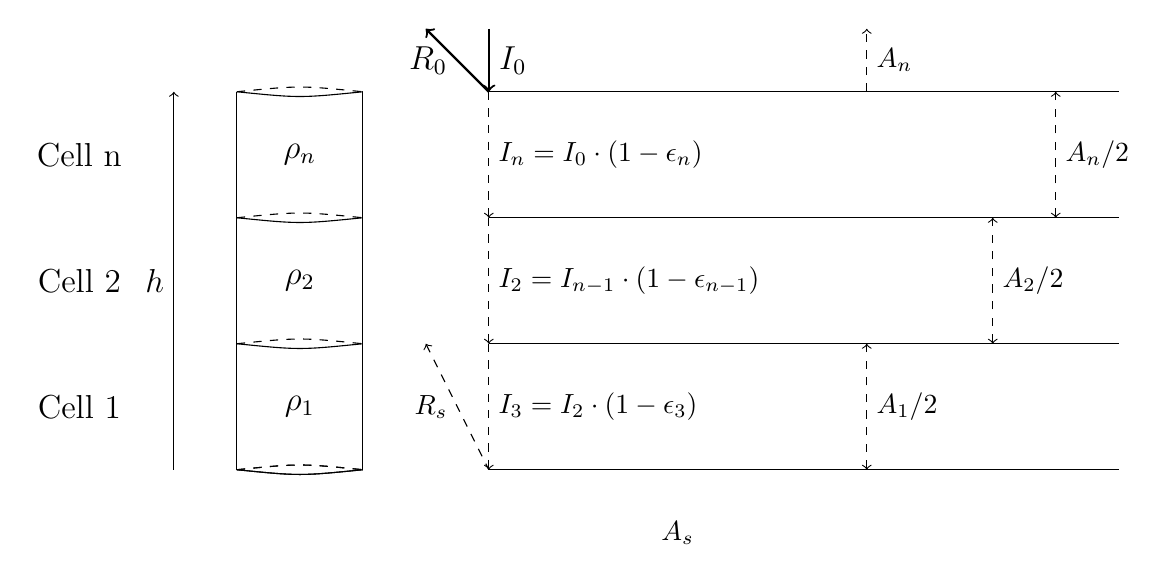
\begin{tikzpicture}[scale = 0.8]
        \draw (0,0) -- (0, 6);
        \draw (2,0) -- (2, 6);

        \draw (0,0)..controls(1,-0.1)..(2, 0);
        \draw[dashed] (0,0)..controls(1,0.1)..(2, 0);

        \draw (0,0)..controls(1,-0.1)..(2, 0);
        \draw[dashed] (0,0)..controls(1,0.1)..(2, 0);

        \draw (0,2)..controls(1, 1.9)..(2, 2);
        \draw[dashed] (0,2)..controls(1,2.1)..(2, 2);

        \draw (0,4)..controls(1, 3.9)..(2, 4);
        \draw[dashed] (0,4)..controls(1,4.1)..(2, 4);

        \draw (0,6)..controls(1, 5.9)..(2, 6);
        \draw[dashed] (0,6)..controls(1,6.1)..(2, 6);

        \node at (-2.5, 1) {\large Cell 1};
        \node at (1, 1) {\large $\rho_1$};

        \node at (-2.5, 3) {\large Cell 2};
        \node at (1, 3) {\large $\rho_2$};

        \node at (-2.5, 5) {\large Cell n};
        \node at (1, 5) {\large $\rho_n$};

        \draw[->] (-1, 0) -- (-1, 6) node[left, pos = 0.5] {\large $h$};

        \draw (4, 0) -- (14, 0);

        \draw (4, 2) -- (14, 2);

        \draw (4, 4) -- (14, 4);

        \draw (4, 6) -- (14, 6);
        \draw[->, thick] (4, 7) -- (4, 6) node[pos = 0.5, right] {\large$I_0$};
        \draw[<-, thick] (3, 7) -- (4, 6) node[pos = 0.5, left] {\large$R_0$};
        \draw[->,dashed] (4, 6) -- (4, 4) node[pos = 0.5, right] { $I_n = I_0\cdot (1-\epsilon_n)$};
        \draw[->,dashed] (4, 4) -- (4, 2) node[pos = 0.5, right] { $I_2 = I_{n - 1}\cdot (1-\epsilon_{n-1})$};
        \draw[<-,dashed] (3, 2) -- (4, 0) node[pos = 0.5, left] { $R_s$ };
        \draw[->,dashed] (4, 2) -- (4, 0) node[pos = 0.5, right] { $I_3 = I_{2}\cdot (1-\epsilon_{3})$};
        \node at ( 7, -1) {$A_s$};
        \draw[<->, dashed] (10, 0) -- (10, 2) node[pos = 0.5, right] {$A_1 / 2$};
        \draw[<->, dashed] (12, 2) -- (12, 4) node[pos = 0.5, right] {$A_2 / 2$};
        \draw[<->, dashed] (13, 4) -- (13, 6) node[pos = 0.5, right] {$A_n / 2$};
        \draw[->, dashed] (10, 6) -- (10, 7) node[pos = 0.5, right] {$A_n $};

    \end{tikzpicture}
    \caption{Schematic of the model}
    \label{fig: model}
\end{figure}\noindent
The densities in each layer is derived from barometric formula, and is thus given by:
\begin{align}
    \rho(z) = \rho_0\cdot\exp\left[\frac{-gMz}{RT_0}\right],\label{eq: density}
\end{align}where $z$ is the height above sea level, $\rho_0$ is the density at sea level, $g$ is the acceleration due to gravity, $M$ is the molar mass of the atmosphere, $R$ is the ideal gas constant, and $T_0$ is the temperature at sea level.
The pressure is given by the same exponential formula but by replacing the constant $\rho_0$ by the pressure at sea level, $P_0$.
From there, we can derive the cross-section for the visible and infra-red radiation as follows:
\begin{align*}
    \sigma^{vis}(z) &= \frac{\alpha_{vis}}{\rho(0)},\\
    \sigma^{inf}(z) &= \frac{\alpha_{inf}}{\rho(0)},
\end{align*}where $\alpha_{vis}$ and $\alpha_{inf}$ are scaling factors.
The model can be solved iteratively, where radiation balance requires that the incoming solar radiation is equal, and its reflection is equal to the outgoing radiation, i.e. $I_0 - \sum_i R_i = A_n$, where $A_n$ is the outgoing radiation from the last cell/space.
The model can thus be described by the following equations:
\begin{align}
    T_i^{\beta} &= \left(T_{i + 1}^{\beta} + \delta_{\beta, inf}\frac{E_{i+1}}{2}\right) \cdot \epsilon_{i}^{\beta}\label{eq: in}\\
    K_i &= \left(K_{i - 1} + \frac{E_{i - 1}}{2}\right)\cdot\epsilon_i^{inf},\label{eq: out}\\
    E_i &= \left(\frac{E_{i + 1} - E_{i - 1}}{2} + K_{i - 1} + T_{i + 1}^{inf}\right)\cdot\left(1 - \epsilon_i^{inf}\right)+T_{i+1}^{vis}\left(1 - \epsilon_i^{vis}\right).\label{eq: energy}
\end{align}In the above equations $T$ is the transmitted radiation $K$ is the outgoing radiation and $E$ is the accumulated energy in the cell, in the notation above $\beta$ is either $vis$ or $inf$.
Note that we can divide the outgoing radiation into two parts, one part that is the reflected radiation in the visible spectrum, and one part that is the emitted radiation in the infra-red spectrum.

\newparagraph
Moreover, in each cell the emitted energy is equal to the absorbed energy, and we assume that each cell emits with equal probability in both directions. This in total leads to a set of seven equations of which must be solved.
The coefficients $\epsilon_i^{\beta}$ are exponential decaying coefficients that describe the transmission in each cell $i$, and are defined by:
\begin{align*}
    \epsilon_i^\beta = \exp\left[-\sigma_i^\beta\rho_i\Delta z\right],
\end{align*}where again $\beta$ is either $vis$ or $inf$. The transmission in each cell then corresponds to the absorption in that cell, i.e. $T_{i+1}^{\beta}(1 - \epsilon_i^{\beta})$, which is what is depicted in the above schematic \ref{fig: model}.

\newparagraph
From the above set of equations, it's possible to find the temperature of each layer by Stefan-Boltzman's law:
\begin{align}
    F = \sigma T^4,\label{eq: stefan-boltzman law}
\end{align}where $\sigma$ is a constant and $T$ is the temperature. The flux, $F$, the net radiation upwards in the cell.
\section{Result \& Discussion}
The above theory was implemented in a Python script.
Below is a table showing the various initial parameters used to solve the system of equations above, eq \eqref{eq: in} -- \eqref{eq: energy}.
\begin{table}[H]
    \centering 
    \caption{Atmosphere parameters}
    \begin{tabular}{|c|c|c|c|c|c|}\hline
        & $P_0$ [kPa] & $T_0$ [K] & $g$ [m$/$s]& $z$ [km] & $I_0$ [W$/$m$^2$] \\\hline
        Earth & $101.3$ & $288$ & $9.81$ & $100$ & $344$ \\\hline
    \end{tabular}
\end{table}\noindent
Using known parameters, such as the pressure at the surface and the gravitational acceleration at the surface, one derived the density and pressure at the different layers.

\begin{figure}[H]
    \centering
    \begin{tikzpicture}
        \begin{axis}[
                xlabel = {Procent},
                ylabel = {Height [m]},
                title = {Atmospheric profile},
                xmin = 0,
                xmax = 1,
            ]
            \addplot[-, mark = o, color = blue] table[x index = 1, y index = 0] {code/layerInfo.dat};
            \addlegendentry{$\rho / \rho_0$};
            \addplot[-, mark = o] table[x index = 2, y index = 0] {code/layerInfo.dat};
            \addlegendentry{$P / P_0$};
        \end{axis}
    \end{tikzpicture}
    \caption{Atmospheric profile of the Earth}
    \label{eq: atmospheric profile of earth}
\end{figure}\noindent
The above figure shows how the normalized pressure and density changes with height. As the height increases, the pressure and density decreases, which is expected.
This indicates that the density and the pressure decreases significantly with height, as compared to temperature which decreases more slowly.

\newparagraph
The surface temperature, is determined by the flux from the surface upwards, and thus is given by $A_s$ is the above schematic \ref{fig: model}, and using eq \eqref{eq: stefan-boltzman law}, we find the surface temperature as a function of number of cells, which is shown below in fig \ref{fig: surface temperature}.
\begin{figure}[H]
    \centering
    \begin{tikzpicture}
        \begin{axis}[
            xlabel = {Number of cells},
            ylabel = {Surface temperature [K]},
            title = {Surface temperature as a function of number of cells},
            ymajorgrids = true,
            xmajorgrids = true,
        ]
        \addplot[] table[x index = 0, y index = 1] {code/ground_temperature2.dat};
        \addplot[domain = 0:100, color = blue] {288} node[above] {$T_0$};
            
        \end{axis}
    \end{tikzpicture}
    \caption{Surface temperature with scaling factors $\alpha_{vis} = 1\cdot10^{-4}$, and $\alpha_{inf} = 1.07\cdot10^{-3}$.}
    \label{fig: surface temperature}
\end{figure}\noindent
We see that the surface-temperature converges towards the true value with increasing number of cells.
This implies that liquid water can exist, and thus as an extension -- life.
The temperature increases inversely proportional to the number of cells, and is thus not highly dependent on the number of cells.
This is expected, as the attenuation in each cell is dependent on the height of the cell, and it's density;
with an increasing number of cells, the height of each cell decreases, but the density is better resolved, and thus the attenuation is better resolved.

\newparagraph
The temperature profile of the earth is shown below in fig \ref{fig: temperature profile}.
As per contrast to the normalized pressure and density, the temperature decreases more slowly with height, as previously mentioned.
This implied that approximations made with the barometric formula, eq \eqref{eq: density}, to some extent, is valid.
Moreover, the temperature profile is plausible, as the temperature decreases with height and converges close to zero at the top of the atmosphere.
This is reasonable, as the temperature of empty space is close to absolute zero, i.e. $0$ K.

\newparagraph
The model was also applied to the planet Venus, and the temperature profile of Venus is shown below in fig \ref{fig: temperature profile venus}.
The following parameters were used to solve the system of equations for Venus\cite{enwiki:1216079584}:
\begin{table}[H]
    \centering 
    \caption{Atmosphere parameters}
    \begin{tabular}{|c|c|c|c|c|c|}\hline
        & $P_0$ [MPa] & $T_0$ [K] & $g$ [m$/$s]& $z$ [km] & $I_0$ [W$/$m$^2$] \\\hline
        Venus & $9.3$ & $737$ & $8.87$ & $250$ & $655.5$ \\\hline
    \end{tabular}
\end{table}\noindent
The scaling factors $\alpha_{vis}$ and $\alpha_{inf}$ were set to $1\cdot10^{-6}$ and $5\cdot10^{-1}$, respectively.
This was done to better approximate Venus dense atmosphere.
Although the attempts to take into account Venus dense atmosphere, the computed surface temperature of Venus is significantly lower than its true surface temperature.
To better approximate, both the Earth's atmosphere and Venus Atmosphere, one would need to take into account the composition of the atmosphere, and the greenhouse effect.
Although our model is simple, and underestimates the temperature of Venus, it still states that the temperature of Venus is significantly higher than the Earth.
This in itself implies that life, as we know it, cannot exist on Venus, since the temperature is too high.

\begin{figure}[H]
    \centering
    \begin{subfigure}{0.45\textwidth}
        \begin{tikzpicture}[scale = 0.75]
            \begin{axis}[ylabel = {Temperature [K]}, xlabel = {Height [km]}, title = {Temperature profile},
                    ymajorgrids = true,
                    xmajorgrids = true,
                    %ytick = {200, 220, 240, 260, 280, 300},
                    %ytick = {10000, 20000, 30000, 40000, 50000, 60000, 80000, 90000, 10000}
                    %xticklabel = {200, 240, 280, 320}
                ]
                \addplot[only marks] table[x index = 0, y index = 1] {code/outputearth.dat};
                \addplot[domain=0:100, color = blue] {288.15} node[below, pos = 0.5] {$T_0$};
            \end{axis}
        \end{tikzpicture}
        \caption{Temperature profile of the Earth}
        \label{fig: temperature profile}
    \end{subfigure}
    \hfill
    \begin{subfigure}{0.45\textwidth}
        \begin{tikzpicture}[scale = 0.75]
            \begin{axis}[ylabel = {Temperature [K]}, xlabel = {Height [km]}, title = {Temperature profile},
                    ymajorgrids = true,
                    xmajorgrids = true,
                    %ytick = {200, 220, 240, 260, 280, 300},
                    %ytick = {10000, 20000, 30000, 40000, 50000, 60000, 80000, 90000, 10000}
                    %xticklabel = {200, 240, 280, 320}
                ]
                \addplot[only marks] table[x index = 0, y index = 1] {code/outputvenus.dat};
                \addplot[domain = 0:250, color = blue] {737} node[below, pos = 0.5] {$T_0$};
            \end{axis}
        \end{tikzpicture}
        \caption{Temperature profile of the Venus}
        \label{fig: temperature profile venus}
    \end{subfigure}
    \caption{Temperature profile of the Earth \ref{fig: temperature profile} and Venus \ref{fig: temperature profile venus}.}
    \label{eq: comparison of temperature profiles}
\end{figure}

\newpage
\section{Conclusion}
The model was able to improve upon the results attained by Stefan-Boltzman's law, by taking into account that the radiation attenuates in the atmosphere and being redistributed.
However, the model is very simple in that the radiation is banded into two categories, visible and infra-red light, instead of being banded into a 'continuous' spectrum.
This would allow for a more accurate representation of the atmosphere, since the different contents of the atmosphere would absorb different wavelengths of radiation.
Moreover, this model does not take into account non-radiant heat transfer, such as convection which is a significant factor in the atmosphere.

\newparagraph
The model was solved iteratively, Appendix \ref{code: submit}, where difficulties arose in the implementation of the model.
The system of equations, eq \eqref{eq: in} -- \eqref{eq: energy}, were not trivial to solve in the sense of being solved 'iteratively'.
Nevertheless, the equations were solved using a simple iterative method, and the results were plausible, with room for improvement.

\printbibliography

\newpage
\section{Appendix}
\lstinputlisting[language = python, caption = {Code for the model}, label={code: submit}]{code/atmosphere.py}
\end{document}
 